\clearpage

\section*{Appendix}
\label{sec:appendix}
% \setcounter{section}{0}   

\section{Dataset Details}
\label{sec:data}

We build our T2T-VICL benchmark by assembling representative paired datasets for a wide set of low-level image processing tasks. For each task we use well-known, publicly available datasets without altering their ground-truth semantics; where appropriate we apply lightweight, clearly documented preprocessing so that training and evaluation are consistent across tasks. The particular dataset selection and provenance mirror those reported in the main paper. The following subsections detail the origin of each dataset, the typical size\slash resolution, and the data split employed in our experiments.

\subsection{Per-Dataset Descriptions}
\noindent \textbf{GOPRO (deblurring).} We use this large motion deblurring dataset introduced for dynamic scene deblurring; it contains 3,214 blurry and sharp pairs captured from high-speed video and typically provided at 1280 $\times$ 720 resolution. This dataset provides realistic, non-uniform motion blur that matches the ``motion-blur restoration'' scenario in our cross-task experiments.

\noindent \textbf{D-HAZY (dehazing).} D-HAZY is a synthetic dehazing dataset produced by applying Koschmieder atmospheric scattering model to images with depth (e.g., images from Middlebury and NYU Depth datasets); it contains on the order of 1,400+ hazy\slash haze-free image pairs and is widely used to benchmark single-image dehazing approaches. We use the official image pairs and follow the commonly used splits reported by the dataset authors.

\noindent \textbf{UHDM (demoireing).} We use the UHDM ultra-high-definition demoireing dataset, which is composed of 5,000 real 4K image pairs collected for moire removal and scale-robust evaluation. UHDM is appropriate for demoireing examples in our benchmark because it contains diverse real-world moire patterns at 4K scale. In practice we downsample/crop to the model's working size for training while retaining high-resolution examples for qualitative figures.

\noindent \textbf{SIDD (denoising).} The Smartphone Image Denoising Dataset (SIDD) provides real noisy smartphone photographs and matching ground truth; the dataset contains roughly $\sim$30,000 noisy images which are generated from multiple scenes and devices and is the standard benchmark for real-world image denoising. We use the released training and benchmark splits for denoising experiments.

\noindent \textbf{RainCityscapes (deraining).} RainCityscapes is built on Cityscapes imagery and provides synthetically generated rainy variants with depth maps; the commonly cited partition includes thousands of rainy/clean images pairs. We use RainCityscapes for deraining A $\rightarrow$ B pairs since it contains realistic outdoor scenes with varying rain density.

\noindent \textbf{iHarmony4 (harmonization).} iHarmony4 is a large image harmonization benchmark composed of four sub-datasets (HCOCO, HAdobe5k, HFlickr, and Hday2night) that together provide tens of thousands of composed images and corresponding real images. We pick the Hday2night set for harmonization experiments.

\noindent \textbf{DIV2K (inpainting, colorization).} DIV2K contains 1,000 high-quality 2K images with a large diversity of contents. For inpainting and colorization experiments we use DIV2K images with controlled masking or decolorization pipelines to create paired inputs and targets as the original images come naturally as the ground truth images.

\noindent \textbf{LoL (light enhancement).} The original LoL (low-light) dataset provides paired low/normal light images; the common LoL-v1 split contains 500 image pairs. We adopt the same pairs and the standard split.

\noindent \textbf{SIR$^2$ (reflection removal).} The SIR$^2$ benchmark provides controlled and wild scenes with ground-truth background/reflection separation. We use the SIR$^2$ ground-truth pairs for reflection removal examples.

\noindent \textbf{ISTD (shadow removal).} The ISTD (Image Shadow Triplets) dataset dataset for shadow understanding contains 1,870 pairs of shadow and shadow-free images. We use the ISTD triplets for all shadow removal A $\rightarrow$ B evaluations.

\noindent \textbf{Night2Day (style transfer).} For style transfer, we use publicly available unpaired dataset commonly referred to as Night2Day, which includes images of outdoor scenes with various appearances such as snow, autumn, dusk, and fog. Depending on the data, we paired images related to the same scene with different appearances ourselves to construct image pairs required for our experiments.

\noindent \textbf{Note on splits \& preprocessing.} For each dataset above we kept the data processing code. Especially for synthetic variants (e.g., DIV2K $\rightarrow$ inpainting/colorization data), we document the exact generation protocol in the dataset code which will be published after this submission.

\subsection{Pair Construction for Cross-Task}
For every source dataset (task A dataset) we sample N examples and pair them with N examples drawn from target dataset (task B dataset) to form cross-task demonstration pairs. To maximize the diversity of implicit descriptions used to teach the sVLM, we generate candidate teacher texts for many different task A/B examples and then apply embedding-based clustering and deduplication to retain high-variance, information-rich implicit prompts.


\section{Prompt Design}
\label{sec:prompt}

Two different conditioning strategies are compared in our experiments: (1) a fixed template prompt that merely describes the I/O demonstration structure (instruction: ``what is shown and what to do''), and (2) implicit prompts generated at inference time by the fine-tuned Qwen student model that describe visual differences and transformation goals between the provided Task A input/output pair and the Task B query input, but crucially without naming tasks explicitly. The implicit prompt therefore acts as a content-dependent, transformation-specific instruction that guides the downstream VLM to adapt the example transformation to the new input. This design is central to T2T-VICL's ability to perform cross-task visual in-context learning.

\subsection{Fixed Prompt}
We used the following fixed prompt as baseline (this is the exact wording used in our fixed-prompt experiments):

\begin{tcolorbox}[colback=gray!20, colframe=gray!20, boxrule=0pt, left=3pt, right=3pt, top=3pt, bottom=3pt]
\emph{This is a visual in-context learning task. The first two images are an input and output of Task A. The third image is the input for Task B. The goal is to perform Task B on the third image and generate an output image, learning from Task A.}
\end{tcolorbox}

\noindent This fixed prompt provides clear structural cues but does not communicate task-specific differences, e.g., whether the change is about removing linear occlusions vs. suppressing uniform noise. Therefore, it acts as a conservative baseline for comparing the benefit of more descriptive (implicit) instructions.

\noindent Similarly, the fixed prompt applied in the same-task VICL for the ablation study is as follows:

\begin{tcolorbox}[colback=gray!20, colframe=gray!20, boxrule=0pt, left=3pt, right=3pt, top=3pt, bottom=3pt]
\emph{This is a visual in-context learning task. The first two images are an input and output of an image processing task. The third image is the input for the SAME task. The goal is to perform this task on the third image and generate an output image, learning from the pair before.}
\end{tcolorbox}

\subsection{Implicit Prompt (Qwen)}
\textbf{How it is created.} For each sampled A $\rightarrow$ B tuple ($I_A^{in}$, $I_A^{l}$, $I_B^{in}, I_B^l$), a large teacher VLM is prompted with four images and an open-ended instruction (``Compare the effects observed in these images and produce a descriptive instruction that would allow another model to transform $I_B^{in}$ into $I_B^{out}$''), which elicits a rich, descriptive text. These candidate texts are post-processed (clustering\slash de-duplication\slash filtering) to keep high-variance, informative implicit prompts which are then used as training targets for our small sVLM (Qwen3-VL-4B) to learn to generate such implicit prompts given similar image triples.

\noindent \textbf{What the implicit prompt contains.} Typical implicit prompts contain three types of information: (1) target goals (what visual attributes should be achieved in the output), (2) input degradation description (what to remove/mitigate), and (3) how to change visual statistics (e.g., preserve texture, restore local contrast, avoid color casts). Importantly the language avoids direct task names (no explicit ``derain/denoise/deblur'' tokens), which forces the model to rely on visual-descriptive cues and allows transferring the transformation style across tasks.

\noindent \textbf{Why it helps.} Because the implicit prompt encodes the target visual change in fine-grained, task-agnostic language, it provides the downstream generator with actionable, content-sensitive guidance. This guidance improves adaptation when the transformation required by Task B differs in surface form from Task A, yet still shares similar latent transformation principles.

\noindent \textbf{Example.}
Below we give one long, representative teacher output used as an illustrative example in the supplementary. This example is intentionally verbose to demonstrate the kinds of distinctions the implicit prompt encodes; a single long instruction like this is used as a training target for sVLM.

\begin{tcolorbox}[colback=gray!20, colframe=gray!20, boxrule=0pt, left=3pt, right=3pt, top=3pt, bottom=3pt]

\emph{This is a visual in-context learning task. The first two images are an input and output of Task A. The third image is the input for Task B. The goal is to perform Task B on the third image and generate an output image, learning from Task A.}
\vspace{1pt}

\emph{\textbf{Analysis of Tasks A and B}}

% \emph{\textbf{Input Image Descriptions}}
\emph{\textbf{Input Descriptions}}

\begin{itemize}

\item \emph{\textbf{Task A:} The input image shows a dimly lit room with stacked boxes containing various items, including a basketball. The lighting is low, making details difficult to discern.}

\item \emph{\textbf{Task B:} The input image is a black-and-white photograph of a person wearing sunglasses and a headscarf, holding a phone to their ear. The image lacks color and has a monochromatic tone.}

\end{itemize}

\emph{\textbf{Visual Changes}}

\begin{itemize}

\item \emph{\textbf{Task A:} The output image is brighter, with improved lighting that enhances visibility and detail of the objects within the room.}

\item \emph{\textbf{Task B:} The output image is in color, transforming the black-and-white photo into a full-color representation, adding vibrancy and depth.}

\end{itemize}

% \emph{\textbf{Differences of Tasks}}
\emph{\textbf{Task Differences}}

\begin{itemize}

\item \emph{\textbf{Task A:} Task A focuses on enhancing brightness and visibility, likely through illumination or contrast adjustments.}

\item \emph{\textbf{Task B:} Task B emphasizes color restoration, converting a grayscale image into a colorful one, which alters the overall aesthetic and provides more visual information.}

\end{itemize}

\end{tcolorbox}

\noindent Similarly, one example of implicitly enhanced prompt in the ablation study section is (Note: same-task VICL does not have the Task Differences item):

\begin{tcolorbox}[colback=gray!20, colframe=gray!20, boxrule=0pt, left=3pt, right=3pt, top=3pt, bottom=3pt]

\emph{This is a visual in-context learning task. The first two images are an input and output of an image processing task. The third image is the input for the same task. The goal is to perform this task on the third image and generate an output image, learning from the pair before.}

\end{tcolorbox}

\begin{tcolorbox}[colback=gray!20, colframe=gray!20, boxrule=0pt, left=3pt, right=3pt, top=3pt, bottom=3pt]

\emph{\textbf{Image Descriptions}}

\emph{Picture 1 shows a monochrome shot of a racer on a motorcycle, while Picture 2 presents the same scene with vibrant, saturated colors restored.}

\emph{\textbf{Visual Changes}}

\emph{The task transforms the grayscale representation into a vivid, full-color depiction, enhancing the visual richness and detail of the subject.}

\emph{The third image, a grayscale kite on grass, would similarly gain vivid color saturation to match the enhanced palette of the first two images.}

\end{tcolorbox}


\section{Inference Details}
\label{sec:infer}

Figure~\ref{fig:fig3} gives a concrete inference-stage example to clarify how the fixed prompt and the implicit prompt are used. Both settings receive the same visual inputs: an input-output demonstration pair from task A and a query input from task B.
T2T-VICL first asks the trained sVLM to produce an implicit prompt from the same images, and the generated prompt is then concatenated with the fixed structural instruction and passed, together with the images, to the frozen VLM.
The figure visualizes this complete route from visual prompt construction to final output, showing why the implicit prompt serves as an interpretable bridge between a task-A demonstration and a task-B query.

\begin{figure*}[t]
    \centering
    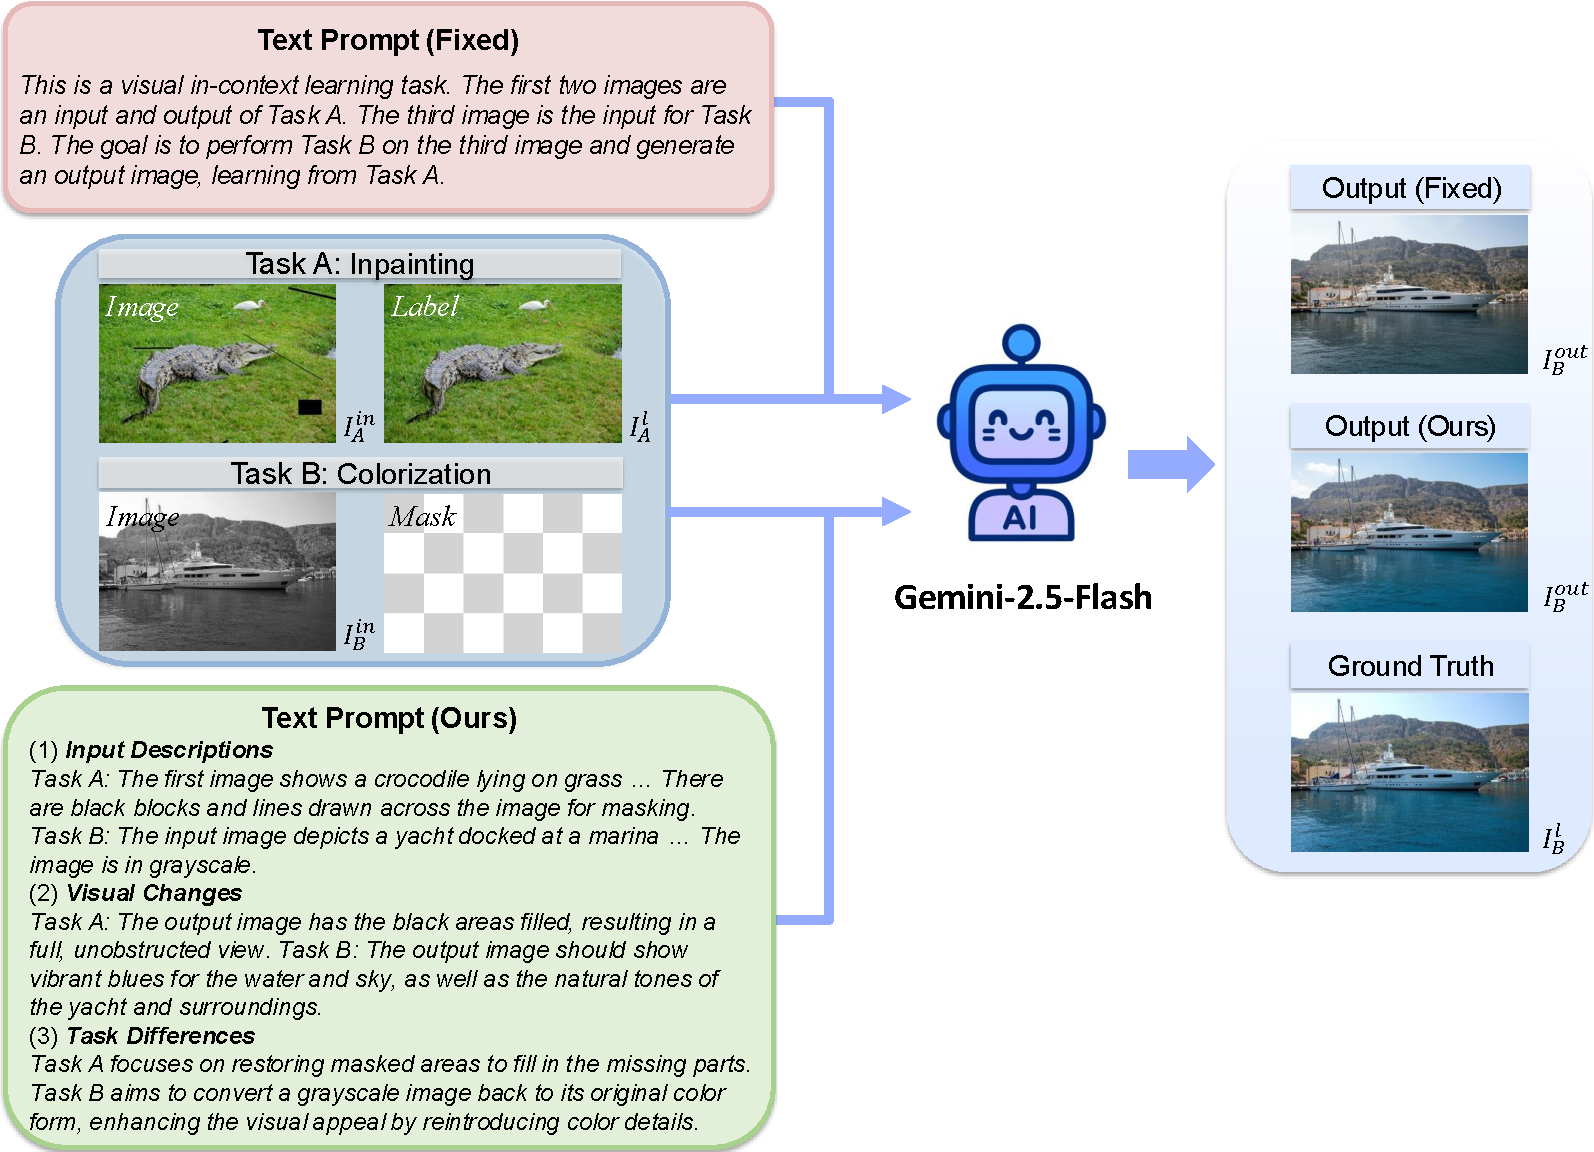
\includegraphics[width=0.9\textwidth]{fig/figure3.pdf}
    \caption{Detailed Example of Cross-Task Visual In-Context Learning in Inference Stage}
    \label{fig:fig3}
\vspace{-8pt}
\end{figure*}


\section{Additional Results and Analysis}

% \subsection{Cross-Task Qualitative Results}
% \label{sec:example}

% \begin{figure*}[ht]
%     \centering
%     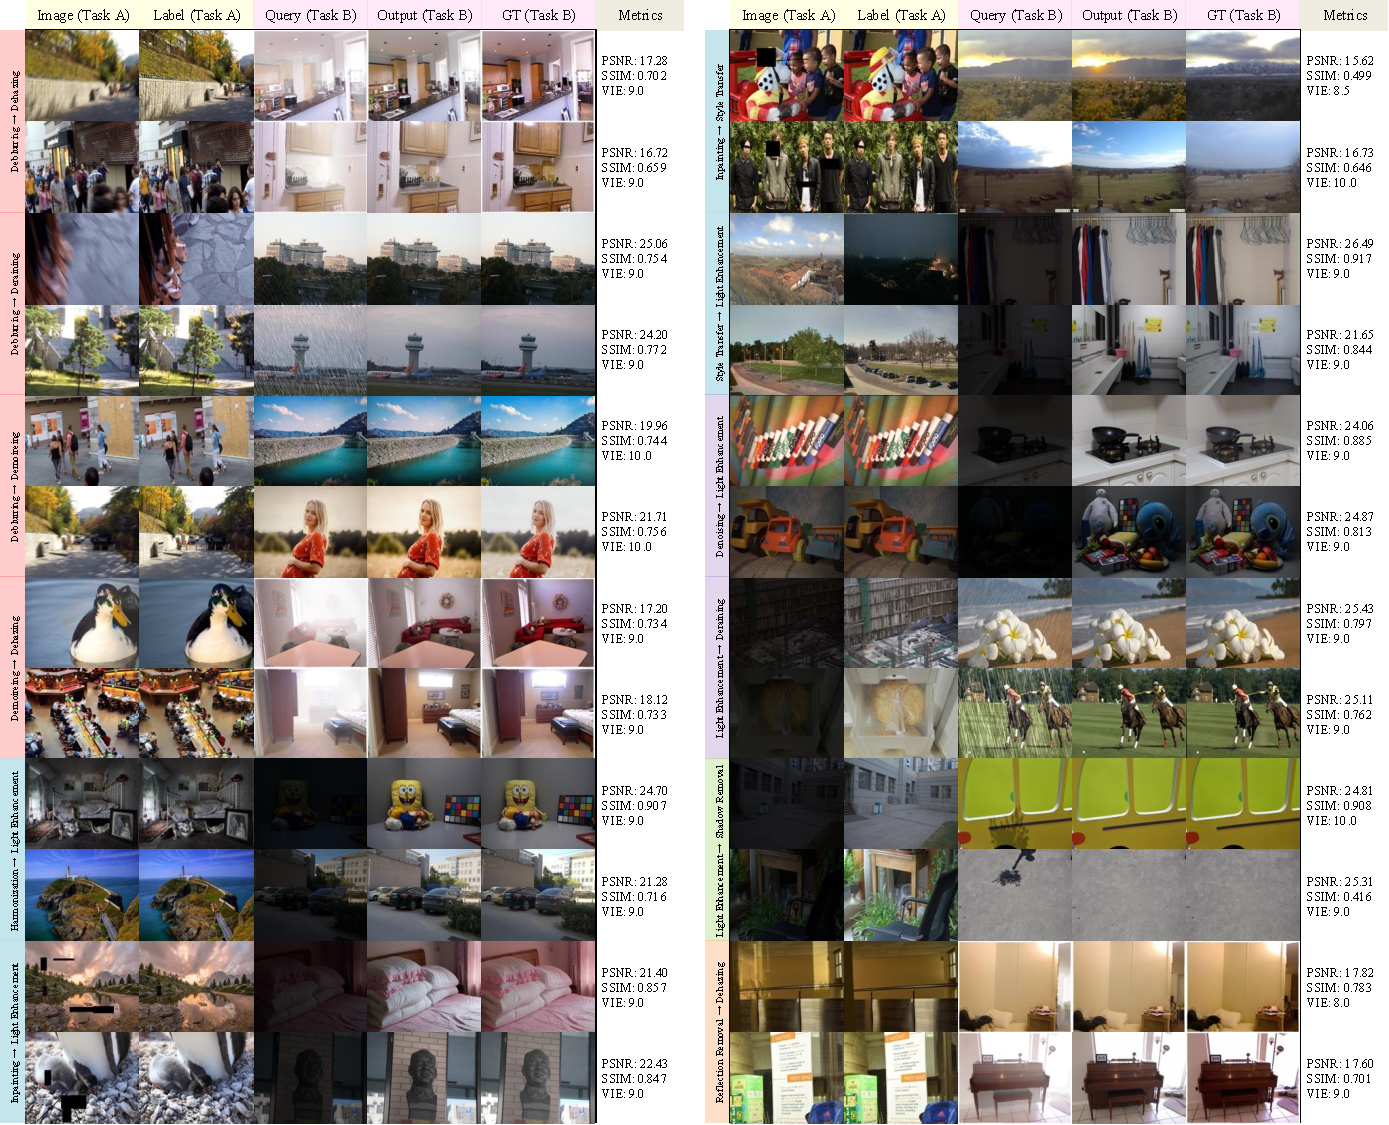
\includegraphics[width=\textwidth]{fig/figure4.pdf}
%     \caption{Representative Examples of Cross-Task In-Context Learning from Gemini in Twelve Pairs}
%     \label{fig:fig4}
% \vspace{-8pt}
% \end{figure*}

% \begin{figure*}[ht]
%     \centering
%     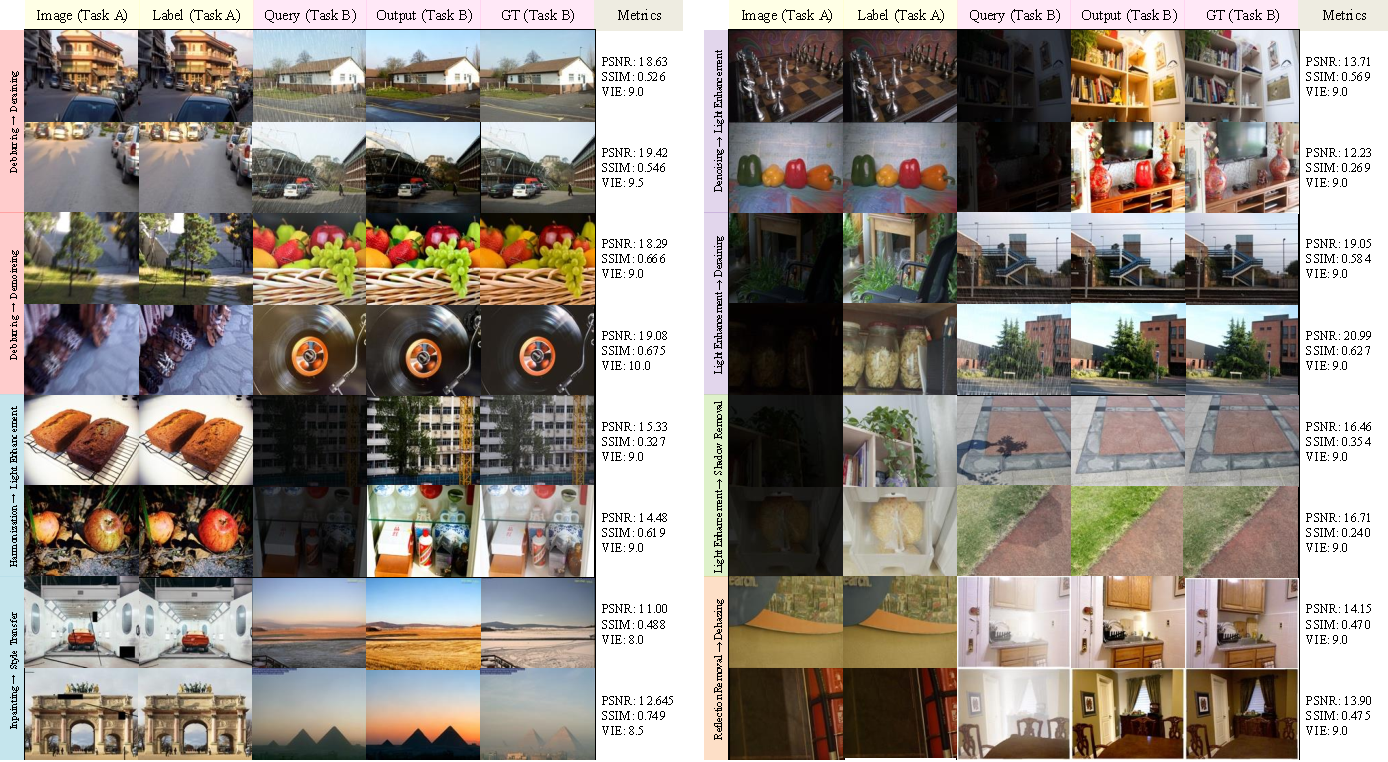
\includegraphics[width=\textwidth]{fig/figure6.pdf}
%     \caption{Representative Examples of Cross-Task In-Context Learning from Seedream in Eight Pairs}
%     \label{fig:fig6}
% \vspace{-8pt}
% \end{figure*}

% The Gemini (see Figure~\ref{fig:fig4}) and Seedream (see Figure~\ref{fig:fig6}) qualitative examples complement the quantitative results in the main paper. They use the same cross-task inference protocol: the fixed prompt and the Qwen-generated implicit prompt are applied to identical task-A demonstrations and task-B queries, while only the final image-editing backbone is changed. The figures illustrate representative examples of cross-task ICL, demonstrating how the VLM adapts flexibly to diverse tasks driven by conditioning implicit text prompts.

\subsection{Cross-Task Results of Seedream}
\label{sec:example}

\begin{figure*}[ht]
    \centering
    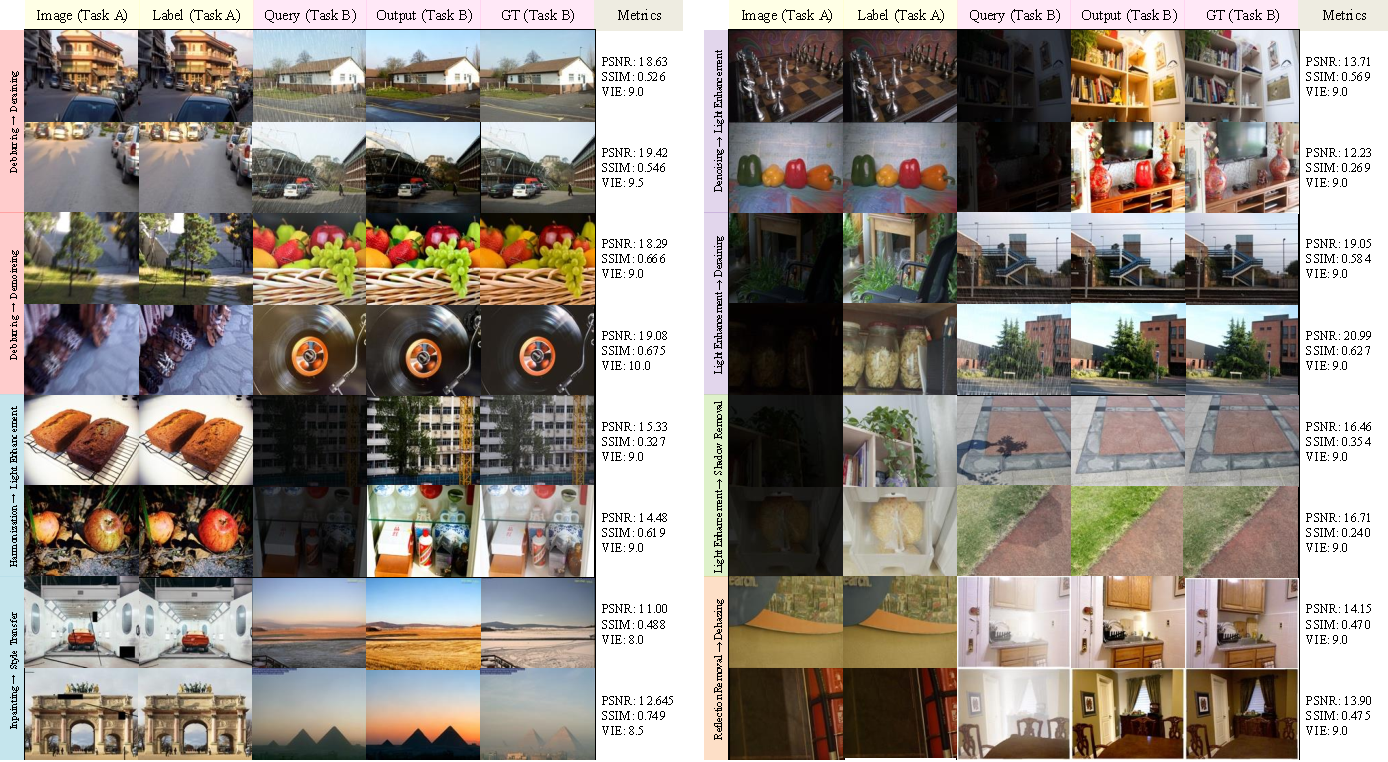
\includegraphics[width=\textwidth]{fig/figure6.pdf}
    \caption{Representative Examples of Cross-Task In-Context Learning from Seedream in Twelve Pairs}
    \label{fig:fig6}
\vspace{-8pt}
\end{figure*}

The Seedream qualitative examples complement the Gemini visual examples in the main paper. They use the same cross-task inference protocol: the fixed prompt and the Qwen-generated implicit prompt are applied to identical task-A demonstrations and task-B queries, while only the final image-editing backbone is changed. These cases are included to show that the qualitative gains of T2T-VICL are not specific to Gemini.


\subsection{Cross-Task Results of Other Models}
The generation ability of our pipeline to other image editing models is presented in Table~\ref{tab:5}. We further include additional open-source models for evaluation, including FLUX.2-dev~\cite{black2025flux}, OmniGen 2~\cite{wu2025omnigen2}, Qwen-Image-Edit~\cite{wu2025qwen, zhao2026qwen}, and FireRed~\cite{team2026firered}. This model choice stems from the VICL setting, in which VLMs accept multiple images and a textual prompt as input to generate a target image. At present, a limited number of any-to-any VLMs support this functionality. These selected VLMs are capable of handling multi-image inputs and generating edited images as outputs. Although different models may exhibit varying strengths across specific tasks, all evaluated models demonstrate a certain degree of cross-task generalization. In terms of overall performance, Gemini-2.5-Flash achieves the highest number of top-tier and second-tier cases across different task-transfer pairs. This observation further validates our choice of Gemini as the final image generation backbone in our framework.

% \begin{table*}[ht]
% \centering
% % \footnotesize
% \scriptsize
% \setlength{\tabcolsep}{0.6pt}
% \renewcommand{\arraystretch}{1.0}

% \captionsetup{width=0.96\textwidth, skip=4pt, type=table}
% \caption{Average of evaluation metrics, generated by baseline models (FLUX 2, OmniGen 2, Qwen-Image) with fixed prompts and Qwen prompts.}
% \vspace{-1pt}

% % \resizebox{\textwidth}{!}{
% \begin{adjustbox}{width=\textwidth}
% % \begin{tabular}{H *{6}{M} G *{6}{M} G *{6}{M}}
% \begin{tabular}{H *{18}{M}}
% \toprule
% \multirow{3}{*}{\textbf{Task}}
% & \multicolumn{6}{c}{\textbf{FLUX.2-dev}}
% & \multicolumn{6}{c}{\textbf{OmniGen 2}}
% & \multicolumn{6}{c}{\textbf{Qwen-Image-Edit}} \\
% % \cmidrule(lr){2-7} \cmidrule(lr){8-13} \cmidrule(lr){14-19}

% & \multicolumn{2}{c}{PSNR}
% & \multicolumn{2}{c}{SSIM}
% & \multicolumn{2}{c}{VIEScore}
% & \multicolumn{2}{c}{PSNR}
% & \multicolumn{2}{c}{SSIM}
% & \multicolumn{2}{c}{VIEScore}
% & \multicolumn{2}{c}{PSNR}
% & \multicolumn{2}{c}{SSIM}
% & \multicolumn{2}{c}{VIEScore} \\

% & \textcolor{gray}{Fix} & \textcolor{gray}{Ours}
% & \textcolor{gray}{Fix} & \textcolor{gray}{Ours}
% & \textcolor{gray}{Fix} & \textcolor{gray}{Ours}
% & \textcolor{gray}{Fix} & \textcolor{gray}{Ours}
% & \textcolor{gray}{Fix} & \textcolor{gray}{Ours}
% & \textcolor{gray}{Fix} & \textcolor{gray}{Ours}
% & \textcolor{gray}{Fix} & \textcolor{gray}{Ours}
% & \textcolor{gray}{Fix} & \textcolor{gray}{Ours}
% & \textcolor{gray}{Fix} & \textcolor{gray}{Ours} \\
% \midrule

% \rowcolor{lightred!30}
% \makecell[l]{Deblurring $\rightarrow$ Dehazing}
% & \cellcolor{lightred!60}8.53 & 8.50
% & 0.196 & \cellcolor{lightred!60}0.217
% & 2.61 & \cellcolor{lightred!60}3.88
% & 7.46 & \cellcolor{lightred!60}7.62
% & 0.175 & \cellcolor{lightred!60}0.183
% & 2.72 & \cellcolor{lightred!60}3.41
% & 8.16 & \cellcolor{lightred!60}8.56
% & 0.183 & \cellcolor{lightred!60}0.238
% & 3.58 & \cellcolor{lightred!60}5.73 \\
% \grayhline

% \rowcolor{lightred!30}
% \makecell[l]{Deblurring $\rightarrow$ Deraining}
% & 9.29 & \cellcolor{lightred!60}9.44
% & 0.160 & \cellcolor{lightred!60}0.162
% & 2.07 & \cellcolor{lightred!60}3.45
% & 8.22 & \cellcolor{lightred!60}8.22
% & \cellcolor{lightred!60}0.132 & 0.126
% & \cellcolor{lightred!60}2.64 & 2.17
% & 10.42 & \cellcolor{lightred!60}10.67
% & 0.188 & \cellcolor{lightred!60}0.234
% & 4.36 & \cellcolor{lightred!60}6.15 \\
% \grayhline

% \rowcolor{lightred!30}
% \makecell[l]{Dehazing $\rightarrow$ Denoising}
% & \cellcolor{lightred!60}8.81 & 8.70
% & \cellcolor{lightred!60}0.498 & 0.483
% & 4.68 & \cellcolor{lightred!60}4.77
% & 6.89 & \cellcolor{lightred!60}7.87
% & \cellcolor{lightred!60}0.404 & 0.403
% & 2.61 & \cellcolor{lightred!60}2.71
% & 11.91 & \cellcolor{lightred!60}15.61
% & 0.487 & \cellcolor{lightred!60}0.597
% & 3.71 & \cellcolor{lightred!60}6.10 \\
% \grayhline

% \rowcolor{lightred!30}
% \makecell[l]{Dehazing $\rightarrow$ Deraining}
% & \cellcolor{lightred!60}9.24 & 8.94
% & \cellcolor{lightred!60}0.207 & 0.205
% & 2.95 & \cellcolor{lightred!60}2.99
% & \cellcolor{lightred!60}7.49 & 7.08
% & \cellcolor{lightred!60}0.158 & 0.148
% & \cellcolor{lightred!60}2.19 & 2.13
% & 8.74 & \cellcolor{lightred!60}11.15
% & 0.177 & \cellcolor{lightred!60}0.276
% & 2.14 & \cellcolor{lightred!60}4.91 \\
% \grayhline

% \rowcolor{lightred!30}
% \makecell[l]{Denoising $\rightarrow$ Deblurring}
% & 10.07 & \cellcolor{lightred!60}10.12
% & \cellcolor{lightred!60}0.287 & 0.241
% & \cellcolor{lightred!60}6.38 & 6.08
% & 8.66 & \cellcolor{lightred!60}9.16
% & 0.273 & \cellcolor{lightred!60}0.280
% & 4.71 & \cellcolor{lightred!60}5.74
% & 9.59 & \cellcolor{lightred!60}10.36
% & 0.244 & \cellcolor{lightred!60}0.295
% & 4.63 & \cellcolor{lightred!60}7.33 \\
% \grayhline

% \rowcolor{lightblue!30}
% \makecell[l]{Colorization $\rightarrow$ Style Transfer}
% & \cellcolor{lightblue!60}9.72 & 8.42
% & \cellcolor{lightblue!60}0.302 & 0.250
% & 5.27 & \cellcolor{lightblue!60}6.42
% & \cellcolor{lightblue!60}7.89 & 7.42
% & \cellcolor{lightblue!60}0.248 & 0.211
% & \cellcolor{lightblue!60}4.13 & 3.44
% & \cellcolor{lightblue!60}9.24 & 9.10
% & 0.245 & \cellcolor{lightblue!60}0.279
% & 6.46 & \cellcolor{lightblue!60}6.54 \\
% \grayhline

% \rowcolor{lightblue!30}
% \makecell[l]{Harmonization $\rightarrow$ Light Enhancement}
% & \cellcolor{lightblue!60}9.09 & 8.32
% & \cellcolor{lightblue!60}0.222 & 0.180
% & \cellcolor{lightblue!60}7.77 & 7.55
% & \cellcolor{lightblue!60}8.32 & 7.34
% & \cellcolor{lightblue!60}0.202 & 0.143
% & 4.79 & \cellcolor{lightblue!60}5.59
% & \cellcolor{lightblue!60}9.32 & 8.85
% & \cellcolor{lightblue!60}0.277 & 0.230
% & 7.23 & \cellcolor{lightblue!60}8.18 \\
% \grayhline

% \rowcolor{lightblue!30}
% \makecell[l]{Inpainting $\rightarrow$ Harmonization}
% & 8.87 & \cellcolor{lightblue!60}9.48
% & 0.186 & \cellcolor{lightblue!60}0.203
% & 5.29 & \cellcolor{lightblue!60}6.39
% & \cellcolor{lightblue!60}7.91 & 7.79
% & \cellcolor{lightblue!60}0.176 & 0.165
% & \cellcolor{lightblue!60}3.32 & 3.16
% & \cellcolor{lightblue!60}10.42 & 10.08
% & \cellcolor{lightblue!60}0.263 & 0.260
% & 6.47 & \cellcolor{lightblue!60}7.09 \\
% \grayhline

% \rowcolor{lightblue!30}
% \makecell[l]{Inpainting $\rightarrow$ Style Transfer}
% & \cellcolor{lightblue!60}9.02 & 8.80
% & \cellcolor{lightblue!60}0.201 & 0.189
% & 2.26 & \cellcolor{lightblue!60}3.78
% & \cellcolor{lightblue!60}8.30 & 7.76
% & \cellcolor{lightblue!60}0.208 & 0.185
% & 3.87 & \cellcolor{lightblue!60}4.10
% & \cellcolor{lightblue!60}9.12 & 9.09
% & 0.207 & \cellcolor{lightblue!60}0.231
% & 4.40 & \cellcolor{lightblue!60}5.00 \\
% \grayhline

% \rowcolor{lightblue!30}
% \makecell[l]{Style Transfer $\rightarrow$ Light Enhancement}
% & \cellcolor{lightblue!60}9.58 & 8.59
% & \cellcolor{lightblue!60}0.289 & 0.245
% & \cellcolor{lightblue!60}6.14 & 6.00
% & \cellcolor{lightblue!60}8.35 & 7.92
% & \cellcolor{lightblue!60}0.232 & 0.186
% & 2.30 & \cellcolor{lightblue!60}3.53
% & \cellcolor{lightblue!60}10.19 & 9.64
% & \cellcolor{lightblue!60}0.318 & 0.281
% & 5.24 & \cellcolor{lightblue!60}6.28 \\
% \grayhline

% \rowcolor{lightyellow!30}
% \makecell[l]{Shadow Removal $\rightarrow$ Reflection Removal}
% & 8.08 & \cellcolor{lightyellow!60}11.73
% & 0.251 & \cellcolor{lightyellow!60}0.344
% & 2.79 & \cellcolor{lightyellow!60}5.37
% & 8.45 & \cellcolor{lightyellow!60}8.99
% & \cellcolor{lightyellow!60}0.226 & 0.215
% & 2.60 & \cellcolor{lightyellow!60}3.16
% & 9.09 & \cellcolor{lightyellow!60}10.78
% & 0.161 & \cellcolor{lightyellow!60}0.318
% & 3.06 & \cellcolor{lightyellow!60}3.93 \\
% \grayhline

% \rowcolor{lightpurple!30}
% \makecell[l]{Denoising $\rightarrow$ Light Enhancement}
% & \cellcolor{lightpurple!60}9.63 & 8.56
% & \cellcolor{lightpurple!60}0.260 & 0.193
% & 7.12 & \cellcolor{lightpurple!60}7.62
% & \cellcolor{lightpurple!60}8.57 & 7.50
% & \cellcolor{lightpurple!60}0.218 & 0.146
% & 6.62 & \cellcolor{lightpurple!60}7.08
% & \cellcolor{lightpurple!60}9.09 & 7.99
% & \cellcolor{lightpurple!60}0.252 & 0.183
% & 5.83 & \cellcolor{lightpurple!60}6.76 \\
% \grayhline

% \rowcolor{lightorange!30}
% \makecell[l]{Reflection Removal $\rightarrow$ Dehazing}
% & 8.77 & \cellcolor{lightorange!50}9.45
% & 0.276 & \cellcolor{lightorange!50}0.308
% & 4.49 & \cellcolor{lightorange!50}5.88
% & \cellcolor{lightorange!50}7.40 & 7.30
% & \cellcolor{lightorange!50}0.241 & 0.236
% & 4.12 & \cellcolor{lightorange!50}4.88
% & \cellcolor{lightorange!50}8.55 & 8.46
% & 0.251 & \cellcolor{lightorange!50}0.270
% & 4.11 & \cellcolor{lightorange!50}6.19 \\
% \grayhline

% \rowcolor{lightorange!30}
% \makecell[l]{Shadow Removal $\rightarrow$ Deraining}
% & 9.00 & \cellcolor{lightorange!50}11.80
% & 0.230 & \cellcolor{lightorange!50}0.261
% & 2.67 & \cellcolor{lightorange!50}4.44
% & 8.02 & \cellcolor{lightorange!50}8.48
% & \cellcolor{lightorange!50}0.146 & 0.134
% & 2.00 & \cellcolor{lightorange!50}2.71
% & 9.89 & \cellcolor{lightorange!50}10.44
% & 0.165 & \cellcolor{lightorange!50}0.213
% & 3.71 & \cellcolor{lightorange!50}3.71 \\

% \bottomrule
% \end{tabular} % }
% \end{adjustbox}
% \end{table*}



\begin{table*}[ht]
\centering
\scriptsize
\setlength{\tabcolsep}{0.5pt}
\renewcommand{\arraystretch}{0.88}
\captionsetup{width=0.98\textwidth, skip=4pt, type=table}
\caption{Average of evaluation metrics for additional backbones, generated by open-source models (FLUX 2, OmniGen 2, Qwen-Image, and FireRed) with fixed prompts and Qwen prompts.}
\vspace{-2pt}
\label{tab:5}

% ---------- (a) ----------
\begin{subtable}[t]{\textwidth}
\centering
\caption{FLUX.2-dev and OmniGen 2}
\vspace{-3pt}
\begin{adjustbox}{width=\textwidth}
\begin{tabular}{>{\raggedright\arraybackslash}m{4cm} *{5}{>{\centering\arraybackslash}m{0.8cm}} >{\centering\arraybackslash}m{1cm} *{5}{>{\centering\arraybackslash}m{0.8cm}} >{\centering\arraybackslash}m{1cm}}
\toprule
\multirow{3}{*}{\textbf{Task}}
& \multicolumn{6}{c}{\textbf{FLUX.2-dev}}
& \multicolumn{6}{c}{\textbf{OmniGen 2}} \\
& \multicolumn{2}{c}{\textbf{PSNR}$\uparrow$}
& \multicolumn{2}{c}{\textbf{SSIM}$\uparrow$}
& \multicolumn{2}{c}{\textbf{VIEScore}$\uparrow$}
& \multicolumn{2}{c}{\textbf{PSNR}$\uparrow$}
& \multicolumn{2}{c}{\textbf{SSIM}$\uparrow$}
& \multicolumn{2}{c}{\textbf{VIEScore}$\uparrow$} \\
& \textcolor{gray}{\textbf{Fixed}} & \textcolor{gray}{\textbf{Ours}}
& \textcolor{gray}{\textbf{Fixed}} & \textcolor{gray}{\textbf{Ours}}
& \textcolor{gray}{\textbf{Fixed}} & \textcolor{gray}{\textbf{Ours}}
& \textcolor{gray}{\textbf{Fixed}} & \textcolor{gray}{\textbf{Ours}}
& \textcolor{gray}{\textbf{Fixed}} & \textcolor{gray}{\textbf{Ours}}
& \textcolor{gray}{\textbf{Fixed}} & \textcolor{gray}{\textbf{Ours}} \\
\midrule
\rowcolor{lightred!30}
Deblurring $\rightarrow$ Dehazing
& \cellcolor{lightred!60}8.53 & 8.50
& 0.196 & \cellcolor{lightred!60}0.217
& 2.61 & \cellcolor{lightred!60}\tabgainsubscript{3.88}{+1.27}
& 7.46 & \cellcolor{lightred!60}7.62
& 0.175 & \cellcolor{lightred!60}0.183
& 2.72 & \cellcolor{lightred!60}\tabgainsubscript{3.41}{+0.69} \\
\grayhline
\rowcolor{lightred!30}
Dehazing $\rightarrow$ Denoising
& \cellcolor{lightred!60}8.81 & 8.70
& \cellcolor{lightred!60}0.498 & 0.483
& 4.68 & \cellcolor{lightred!60}\tabgainsubscript{4.77}{+0.09}
& 6.89 & \cellcolor{lightred!60}7.87
& \cellcolor{lightred!60}0.404 & 0.403
& 2.61 & \cellcolor{lightred!60}\tabgainsubscript{2.71}{+0.10} \\
\grayhline
\rowcolor{lightred!30}
Deraining $\rightarrow$ Demoireing
& \cellcolor{lightred!60}9.51 & 8.99
& \cellcolor{lightred!60}0.461 & 0.444
& \cellcolor{lightred!60}5.05 & \tablosssubscript{5.03}{-0.02}
& 7.40 & \cellcolor{lightred!60}7.55
& 0.373 & \cellcolor{lightred!60}0.375
& 2.66 & \cellcolor{lightred!60}\tabgainsubscript{2.98}{+0.32} \\
\grayhline
\rowcolor{lightblue!30}
Harmonization $\rightarrow$ Style Transfer
& \cellcolor{lightblue!60}9.07 & 8.83
& \cellcolor{lightblue!60}0.253 & 0.246
& 2.95 & \cellcolor{lightblue!60}\tabgainsubscript{5.68}{+2.73}
& \cellcolor{lightblue!60}8.44 & 7.84
& \cellcolor{lightblue!60}0.251 & 0.227
& 5.03 & \cellcolor{lightblue!60}\tabsamesubscript{5.03}{+0.00} \\
\grayhline
\rowcolor{lightblue!30}
Inpainting $\rightarrow$ Style Transfer
& \cellcolor{lightblue!60}9.02 & 8.80
& \cellcolor{lightblue!60}0.201 & 0.189
& 2.26 & \cellcolor{lightblue!60}\tabgainsubscript{3.78}{+1.52}
& \cellcolor{lightblue!60}8.30 & 7.76
& \cellcolor{lightblue!60}0.208 & 0.185
& 3.87 & \cellcolor{lightblue!60}\tabgainsubscript{4.10}{+0.23} \\
\grayhline
\rowcolor{lightyellow!30}
Shadow Removal $\rightarrow$ Reflection Removal
& 8.08 & \cellcolor{lightyellow!60}11.73
& 0.251 & \cellcolor{lightyellow!60}0.344
& 2.79 & \cellcolor{lightyellow!60}\tabgainsubscript{5.37}{+2.58}
& 8.45 & \cellcolor{lightyellow!60}8.99
& \cellcolor{lightyellow!60}0.226 & 0.215
& 2.60 & \cellcolor{lightyellow!60}\tabgainsubscript{3.16}{+0.56} \\
\grayhline
\rowcolor{lightpurple!30}
Denoising $\rightarrow$ Light Enhancement
& \cellcolor{lightpurple!60}9.63 & 8.56
& \cellcolor{lightpurple!60}0.260 & 0.193
& 7.12 & \cellcolor{lightpurple!60}\tabgainsubscript{7.62}{+0.50}
& \cellcolor{lightpurple!60}8.57 & 7.50
& \cellcolor{lightpurple!60}0.218 & 0.146
& 6.62 & \cellcolor{lightpurple!60}\tabgainsubscript{7.08}{+0.46} \\
\grayhline
\rowcolor{lightorange!30}
Reflection Removal $\rightarrow$ Dehazing
& 8.77 & \cellcolor{lightorange!50}9.45
& 0.276 & \cellcolor{lightorange!50}0.308
& 4.49 & \cellcolor{lightorange!50}\tabgainsubscript{5.88}{+1.39}
& \cellcolor{lightorange!50}7.40 & 7.30
& \cellcolor{lightorange!50}0.241 & 0.236
& 4.12 & \cellcolor{lightorange!50}\tabgainsubscript{4.88}{+0.76} \\
\grayhline
\rowcolor{lightorange!30}
Shadow Removal $\rightarrow$ Deraining
& 9.00 & \cellcolor{lightorange!50}11.80
& 0.230 & \cellcolor{lightorange!50}0.261
& 2.67 & \cellcolor{lightorange!50}\tabgainsubscript{4.44}{+1.77}
& 8.02 & \cellcolor{lightorange!50}8.48
& \cellcolor{lightorange!50}0.146 & 0.134
& 2.00 & \cellcolor{lightorange!50}\tabgainsubscript{2.71}{+0.71} \\
\bottomrule
\end{tabular}
\end{adjustbox}
\end{subtable}

\vspace{3pt}

\begin{subtable}[t]{\textwidth}
\centering
\caption{Qwen-Image-Edit-2511 and FireRed-Image-Edit-1.1}
\vspace{-3pt}
\begin{adjustbox}{width=\textwidth}
\begin{tabular}{>{\raggedright\arraybackslash}m{4cm} *{5}{>{\centering\arraybackslash}m{0.8cm}} >{\centering\arraybackslash}m{1cm} *{5}{>{\centering\arraybackslash}m{0.8cm}} >{\centering\arraybackslash}m{1cm}}
\toprule
\multirow{3}{*}{\textbf{Task}}
& \multicolumn{6}{c}{\textbf{Qwen-Image-Edit}}
& \multicolumn{6}{c}{\textbf{FireRed-Image-Edit}} \\
& \multicolumn{2}{c}{\textbf{PSNR}$\uparrow$}
& \multicolumn{2}{c}{\textbf{SSIM}$\uparrow$}
& \multicolumn{2}{c}{\textbf{VIEScore}$\uparrow$}
& \multicolumn{2}{c}{\textbf{PSNR}$\uparrow$}
& \multicolumn{2}{c}{\textbf{SSIM}$\uparrow$}
& \multicolumn{2}{c}{\textbf{VIEScore}$\uparrow$} \\
& \textcolor{gray}{\textbf{Fixed}} & \textcolor{gray}{\textbf{Ours}}
& \textcolor{gray}{\textbf{Fixed}} & \textcolor{gray}{\textbf{Ours}}
& \textcolor{gray}{\textbf{Fixed}} & \textcolor{gray}{\textbf{Ours}}
& \textcolor{gray}{\textbf{Fixed}} & \textcolor{gray}{\textbf{Ours}}
& \textcolor{gray}{\textbf{Fixed}} & \textcolor{gray}{\textbf{Ours}}
& \textcolor{gray}{\textbf{Fixed}} & \textcolor{gray}{\textbf{Ours}} \\
\midrule
\rowcolor{lightred!30}
Deblurring $\rightarrow$ Dehazing
& 8.16 & \cellcolor{lightred!60}8.56
& 0.183 & \cellcolor{lightred!60}0.238
& 3.58 & \cellcolor{lightred!60}\tabgainsubscript{5.73}{+2.15}
& \cellcolor{lightred!60}8.90 & 8.27
& \cellcolor{lightred!60}0.260 & 0.178
& 6.16 & \cellcolor{lightred!60}\tabgainsubscript{6.46}{+0.30} \\
\grayhline
\rowcolor{lightred!30}
Deblurring $\rightarrow$ Deraining
& 10.42 & \cellcolor{lightred!60}10.67
& 0.188 & \cellcolor{lightred!60}0.234
& 4.36 & \cellcolor{lightred!60}\tabgainsubscript{6.15}{+1.79}
& \cellcolor{lightred!60}9.35 & 8.92
& \cellcolor{lightred!60}0.164 & 0.139
& 5.20 & \cellcolor{lightred!60}\tabgainsubscript{6.21}{+1.01} \\
\grayhline
\rowcolor{lightred!30}
Dehazing $\rightarrow$ Denoising
& 11.91 & \cellcolor{lightred!60}15.61
& 0.487 & \cellcolor{lightred!60}0.597
& 3.71 & \cellcolor{lightred!60}\tabgainsubscript{6.10}{+2.39}
& 7.87 & \cellcolor{lightred!60}9.09
& 0.457 & \cellcolor{lightred!60}0.473
& 5.78 & \cellcolor{lightred!60}\tabgainsubscript{6.03}{+0.25} \\
\grayhline
\rowcolor{lightred!30}
Dehazing $\rightarrow$ Deraining
& 8.74 & \cellcolor{lightred!60}11.15
& 0.177 & \cellcolor{lightred!60}0.276
& 2.14 & \cellcolor{lightred!60}\tabgainsubscript{4.91}{+2.77}
& 8.56 & \cellcolor{lightred!60}8.68
& \cellcolor{lightred!60}0.193 & 0.181
& 3.08 & \cellcolor{lightred!60}\tabgainsubscript{3.94}{+0.86} \\
\grayhline
\rowcolor{lightred!30}
Demoireing $\rightarrow$ Dehazing
& 8.54 & \cellcolor{lightred!60}8.57
& 0.229 & \cellcolor{lightred!60}0.271
& 4.07 & \cellcolor{lightred!60}\tabgainsubscript{5.31}{+1.24}
& 8.71 & \cellcolor{lightred!60}9.23
& 0.276 & \cellcolor{lightred!60}0.294
& 5.41 & \cellcolor{lightred!60}\tabgainsubscript{6.16}{+0.75} \\
\grayhline
\rowcolor{lightred!30}
Denoising $\rightarrow$ Deblurring
& 9.59 & \cellcolor{lightred!60}10.36
& 0.244 & \cellcolor{lightred!60}0.295
& 4.63 & \cellcolor{lightred!60}\tabgainsubscript{7.33}{+2.70}
& 9.72 & \cellcolor{lightred!60}9.99
& 0.263 & \cellcolor{lightred!60}0.293
& 7.13 & \cellcolor{lightred!60}\tabgainsubscript{8.49}{+1.36} \\
\grayhline
\rowcolor{lightblue!30}
Colorization $\rightarrow$ Style Transfer
& \cellcolor{lightblue!60}9.24 & 9.10
& 0.245 & \cellcolor{lightblue!60}0.279
& 6.46 & \cellcolor{lightblue!60}\tabgainsubscript{6.54}{+0.08}
& \cellcolor{lightblue!60}8.75 & 8.46
& \cellcolor{lightblue!60}0.262 & 0.235
& 7.10 & \cellcolor{lightblue!60}\tabgainsubscript{7.90}{+0.80} \\
\grayhline
\rowcolor{lightblue!30}
Harmonization $\rightarrow$ Light Enhancement
& \cellcolor{lightblue!60}9.32 & 8.85
& \cellcolor{lightblue!60}0.277 & 0.230
& 7.23 & \cellcolor{lightblue!60}\tabgainsubscript{8.18}{+0.95}
& \cellcolor{lightblue!60}8.97 & 8.77
& \cellcolor{lightblue!60}0.225 & 0.205
& 8.14 & \cellcolor{lightblue!60}\tabgainsubscript{8.33}{+0.19} \\
\grayhline
\rowcolor{lightblue!30}
Inpainting $\rightarrow$ Style Transfer
& \cellcolor{lightblue!60}9.12 & 9.09
& 0.207 & \cellcolor{lightblue!60}0.231
& 4.40 & \cellcolor{lightblue!60}\tabgainsubscript{5.00}{+0.60}
& \cellcolor{lightblue!60}9.08 & 8.82
& \cellcolor{lightblue!60}0.211 & 0.198
& 4.12 & \cellcolor{lightblue!60}\tabgainsubscript{5.08}{+0.96} \\
\grayhline
\rowcolor{lightyellow!30}
Shadow Removal $\rightarrow$ Reflection Removal
& 9.09 & \cellcolor{lightyellow!60}10.78
& 0.161 & \cellcolor{lightyellow!60}0.318
& 3.06 & \cellcolor{lightyellow!60}\tabgainsubscript{3.93}{+0.87}
& \cellcolor{lightyellow!60}9.11 & 8.43
& \cellcolor{lightyellow!60}0.226 & 0.210
& 3.35 & \cellcolor{lightyellow!60}\tabgainsubscript{3.55}{+0.20} \\
\grayhline
\rowcolor{lightpurple!30}
Denoising $\rightarrow$ Light Enhancement
& \cellcolor{lightpurple!60}9.09 & 7.99
& \cellcolor{lightpurple!60}0.252 & 0.183
& 5.83 & \cellcolor{lightpurple!60}\tabgainsubscript{6.76}{+0.93}
& \cellcolor{lightpurple!60}9.60 & 9.22
& \cellcolor{lightpurple!60}0.254 & 0.224
& 8.64 & \cellcolor{lightpurple!60}\tabgainsubscript{8.70}{+0.06} \\
\grayhline
\rowcolor{lightpurple!30}
Light Enhancement $\rightarrow$ Deraining
& 9.51 & \cellcolor{lightpurple!60}10.07
& 0.203 & \cellcolor{lightpurple!60}0.231
& 3.47 & \cellcolor{lightpurple!60}\tabgainsubscript{3.48}{+0.01}
& \cellcolor{lightpurple!60}9.08 & 8.80
& \cellcolor{lightpurple!60}0.191 & 0.177
& 5.23 & \cellcolor{lightpurple!60}\tabgainsubscript{5.41}{+0.18} \\
\grayhline
\rowcolor{lightorange!30}
Reflection Removal $\rightarrow$ Dehazing
& \cellcolor{lightorange!50}8.55 & 8.46
& 0.251 & \cellcolor{lightorange!50}0.270
& 4.11 & \cellcolor{lightorange!50}\tabgainsubscript{6.19}{+2.08}
& \cellcolor{lightorange!50}8.53 & 8.18
& \cellcolor{lightorange!50}0.277 & 0.240
& 6.50 & \cellcolor{lightorange!50}\tabgainsubscript{7.55}{+1.05} \\
\grayhline
\rowcolor{lightorange!30}
Shadow Removal $\rightarrow$ Deraining
& 9.89 & \cellcolor{lightorange!50}10.44
& 0.165 & \cellcolor{lightorange!50}0.213
& 3.71 & \cellcolor{lightorange!50}\tabsamesubscript{3.71}{+0.00}
& \cellcolor{lightorange!50}10.01 & 8.87
& \cellcolor{lightorange!50}0.191 & 0.173
& 3.85 & \cellcolor{lightorange!50}\tabgainsubscript{4.07}{+0.22} \\
\bottomrule
\end{tabular}
\end{adjustbox}
\end{subtable}

\vspace{-6pt}
\end{table*}



\subsection{Second-Tier Typed Result Explanation}
\label{sec:viescore}

The second-tier group contains task pairs where T2T-VICL consistently improves VIEScore, while PSNR or SSIM may decrease. We may not interpret these cases as failures of cross-task VICL, as the visual consistency of most generated results remains comparable to those in the top-tier group (see Figure~\ref{fig:fig5}). The gap instead might indicate a mismatch between pixel-aligned fidelity metrics and the goal of several specific target tasks, especially when the target task is closer to conditional generation than deterministic restoration. This issue is especially clear for colorization and style transfer, which have inherent one-to-many ambiguity: multiple plausible outputs may correspond to the same input~\cite{su2020instance,kang2023ddcolor}.

\begin{figure*}[ht]
    \centering
    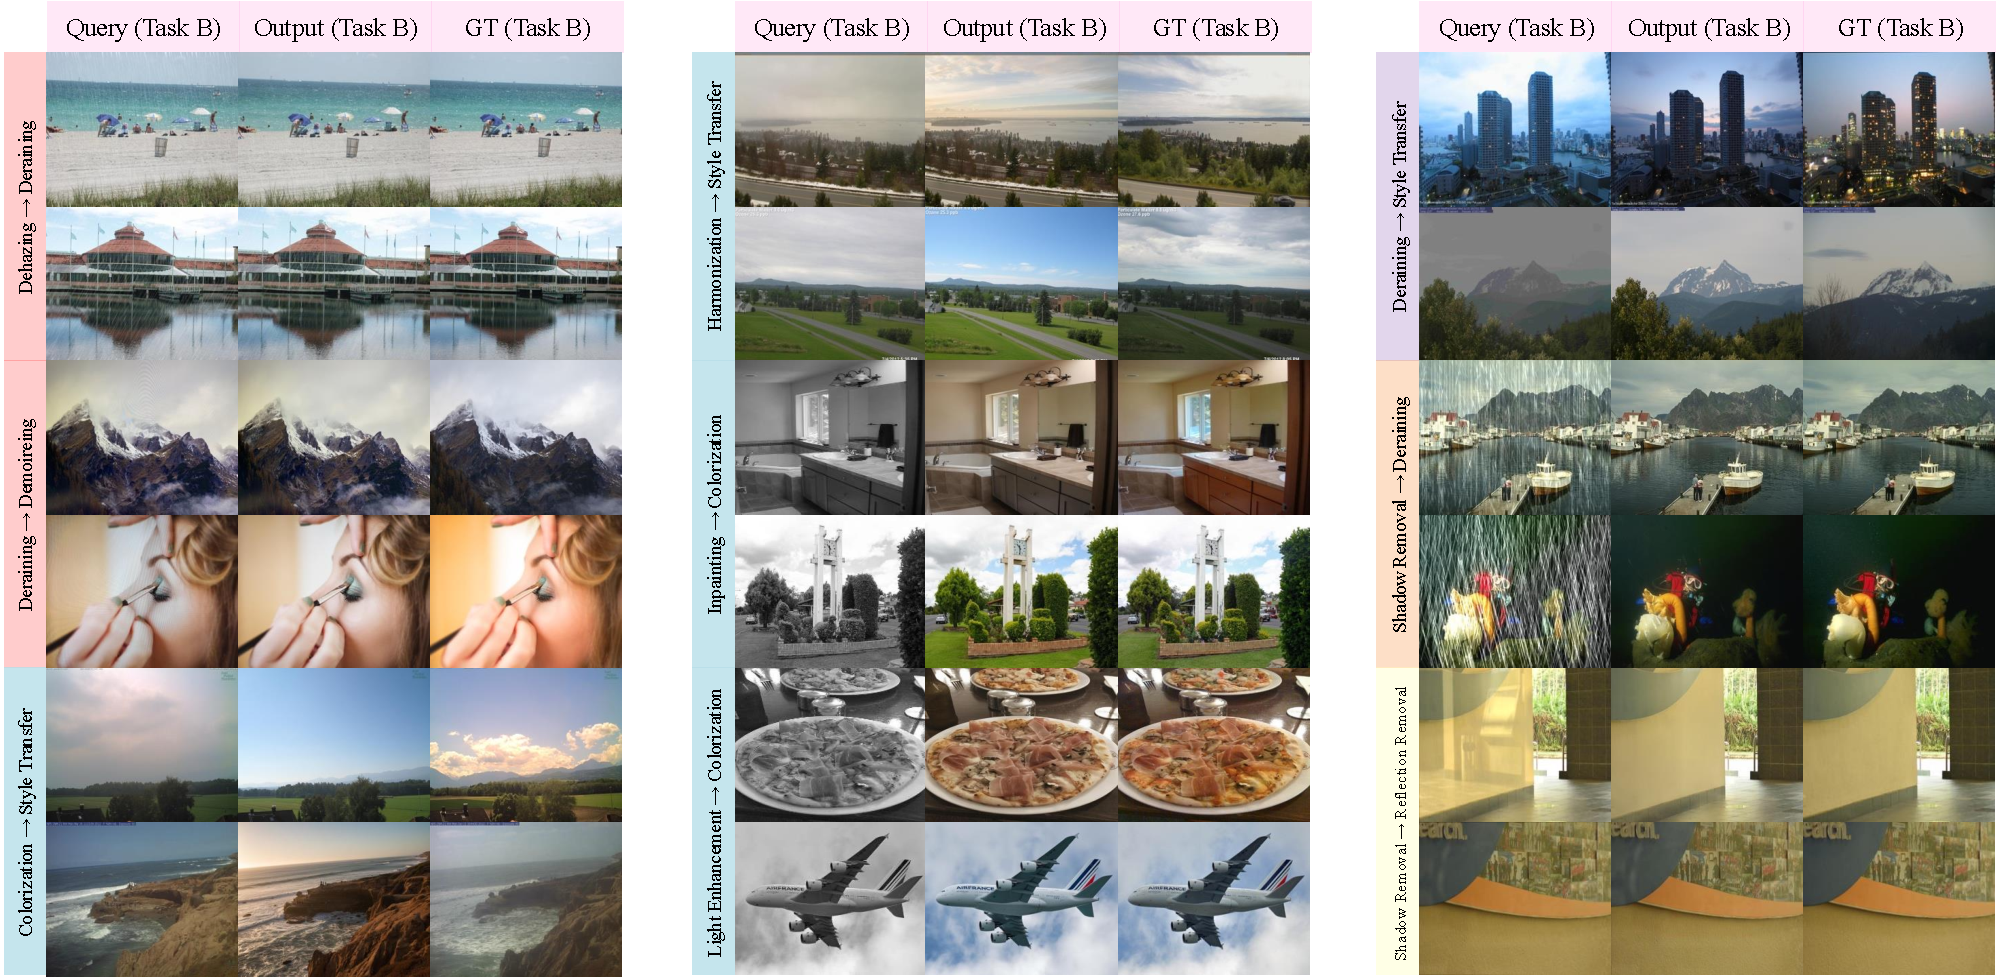
\includegraphics[width=\textwidth]{fig/figure5.pdf}
    \caption{Representative Examples of Cross-Task In-Context Learning from Gemini in Nine Pairs}
    \label{fig:fig5}
\vspace{-8pt}
\end{figure*}

In colorization, an output that remains close to the grayscale input can preserve luminance structure and obtain competitive PSNR or SSIM, even if it fails to add plausible chroma. Recent colorization studies still commonly report PSNR and SSIM, but they increasingly supplement them with perceptual, distributional, or color-statistical measures such as LPIPS, FID, and colorfulness-related metrics~\cite{wu2021towards,kang2023ddcolor}. This is not because PSNR/SSIM are invalid, but because pixel-level fidelity alone cannot fully capture color plausibility under a one-to-many target distribution. A VIEScore improvement with a small PSNR/SSIM drop can therefore still correspond to better task performance.

Style transfer has an even weaker one-to-one correspondence assumption: a successful stylized image should preserve semantic content while intentionally changing appearance, texture, and color statistics. Accordingly, style-transfer studies often report perceptual measures and human preference evaluation rather than solely PSNR or SSIM metrics~\cite{deng2022stytr2, wright2022artfid}.

These related observations actually support our use of VIEScore as the primary signal for the second-tier group, because VIEScore is able to evaluate whether the output follows the intended visual instruction and preserves the relevant content. The consistent superiority of VIEScore over IQA metrics in the second-tier group suggests that our approach prioritizes semantic preservation and cross-task coherence.

To complement the PSNR/SSIM-based analysis, we evaluate all task pairs whose target task is colorization, style transfer, or deraining using perceptual, distributional, and color-aware metrics. Table~\ref{tab:new-metrics} reports Fixed and Ours side by side for each backbone; lower values indicate better agreement with the task-B ground truth or target distribution. CIEDE2000 is used only for colorization/style-transfer targets, ArtFID only for style-transfer targets, and deraining-target rows are evaluated with LPIPS, DISTS, and FID.

\begin{table*}[t]
\centering
\scriptsize
\setlength{\tabcolsep}{2.8pt}
\caption{Additional evaluation metrics for targeted task pairs. All metrics are lower-is-better; within each Fixed/Ours pair, the lower value is shown in bold. CIEDE2000 is reported only for target tasks involving colorization or style transfer, and ArtFID is reported only when the target task is style transfer.}
\label{tab:new-metrics}
\resizebox{\textwidth}{!}{%
\begin{tabular}{lcccccccccc}
\toprule
\multicolumn{11}{c}{\textbf{Gemini 2.5 Flash}} \\
\midrule
\multirow{2}{*}{Task Pair} & \multicolumn{2}{c}{CIEDE$\downarrow$} & \multicolumn{2}{c}{LPIPS$\downarrow$} & \multicolumn{2}{c}{DISTS$\downarrow$} & \multicolumn{2}{c}{FID$\downarrow$} & \multicolumn{2}{c}{ArtFID$\downarrow$} \\
\cmidrule(lr){2-3}\cmidrule(lr){4-5}\cmidrule(lr){6-7}\cmidrule(lr){8-9}\cmidrule(lr){10-11}
 & Fixed & Ours & Fixed & Ours & Fixed & Ours & Fixed & Ours & Fixed & Ours \\
\midrule
Deblurring $\rightarrow$ Deraining & -- & -- & 0.226 & \textbf{0.194} & 0.158 & \textbf{0.138} & 79.3 & \textbf{63.3} & -- & -- \\
Dehazing $\rightarrow$ Deraining & -- & -- & 0.219 & \textbf{0.204} & 0.150 & \textbf{0.139} & 80.3 & \textbf{73.6} & -- & -- \\
Colorization $\rightarrow$ Style Transfer & \textbf{18.56} & 19.81 & 0.522 & \textbf{0.520} & 0.242 & \textbf{0.239} & 98.5 & \textbf{97.5} & \textbf{100.2} & 102.4 \\
Harmonization $\rightarrow$ Style Transfer & \textbf{19.00} & 19.50 & 0.550 & \textbf{0.530} & 0.264 & \textbf{0.246} & 117.5 & \textbf{102.4} & 105.8 & \textbf{100.1} \\
Inpainting $\rightarrow$ Colorization & 10.63 & \textbf{10.60} & 0.247 & \textbf{0.209} & 0.165 & \textbf{0.144} & 97.9 & \textbf{80.8} & -- & -- \\
Inpainting $\rightarrow$ Style Transfer & 28.87 & \textbf{19.23} & 0.796 & \textbf{0.508} & 0.443 & \textbf{0.236} & 274.4 & \textbf{99.3} & 284.5 & \textbf{98.3} \\
Light Enhancement $\rightarrow$ Colorization & \textbf{9.83} & 10.24 & 0.219 & \textbf{0.206} & 0.152 & \textbf{0.141} & 91.8 & \textbf{78.4} & -- & -- \\
Deraining $\rightarrow$ Style Transfer & \textbf{18.44} & 19.18 & 0.574 & \textbf{0.524} & 0.269 & \textbf{0.236} & 121.2 & \textbf{99.8} & 126.0 & \textbf{103.9} \\
Light Enhancement $\rightarrow$ Deraining & -- & -- & 0.274 & \textbf{0.179} & 0.189 & \textbf{0.127} & 109.0 & \textbf{58.2} & -- & -- \\
Shadow Removal $\rightarrow$ Deraining & -- & -- & 0.202 & \textbf{0.198} & 0.143 & \textbf{0.139} & 69.3 & \textbf{64.7} & -- & -- \\
\bottomrule
\end{tabular}%
}
\vspace{0.6em}
\resizebox{\textwidth}{!}{%
\begin{tabular}{lcccccccccc}
\toprule
\multicolumn{11}{c}{\textbf{Seedream 4.0}} \\
\midrule
\multirow{2}{*}{Task Pair} & \multicolumn{2}{c}{CIEDE$\downarrow$} & \multicolumn{2}{c}{LPIPS$\downarrow$} & \multicolumn{2}{c}{DISTS$\downarrow$} & \multicolumn{2}{c}{FID$\downarrow$} & \multicolumn{2}{c}{ArtFID$\downarrow$} \\
\cmidrule(lr){2-3}\cmidrule(lr){4-5}\cmidrule(lr){6-7}\cmidrule(lr){8-9}\cmidrule(lr){10-11}
 & Fixed & Ours & Fixed & Ours & Fixed & Ours & Fixed & Ours & Fixed & Ours \\
\midrule
Deblurring $\rightarrow$ Deraining & -- & -- & 0.414 & \textbf{0.398} & 0.250 & \textbf{0.239} & 135.9 & \textbf{113.8} & -- & -- \\
Dehazing $\rightarrow$ Deraining & -- & -- & 0.371 & \textbf{0.357} & \textbf{0.228} & 0.229 & 119.2 & \textbf{112.5} & -- & -- \\
Colorization $\rightarrow$ Style Transfer & \textbf{28.40} & 29.21 & 0.629 & \textbf{0.623} & 0.297 & \textbf{0.295} & 113.2 & \textbf{103.0} & 139.1 & \textbf{132.5} \\
Light Enhancement $\rightarrow$ Colorization & 23.39 & \textbf{22.82} & 0.412 & \textbf{0.383} & 0.223 & \textbf{0.208} & 130.3 & \textbf{103.7} & -- & -- \\
Light Enhancement $\rightarrow$ Deraining & -- & -- & 0.398 & \textbf{0.364} & 0.255 & \textbf{0.228} & 131.6 & \textbf{104.4} & -- & -- \\
\bottomrule
\end{tabular}%
}
\end{table*}
